\chapter{Implementacija i korisničko sučelje}
		
		
		\section{Korištene tehnologije i alati}
		
			\textbf{\textit{dio 2. revizije}}
			
			 \textit{Detaljno navesti sve tehnologije i alate koji su primijenjeni pri izradi dokumentacije i aplikacije. Ukratko ih opisati, te navesti njihovo značenje i mjesto primjene. Za svaki navedeni alat i tehnologiju je potrebno \textbf{navesti internet poveznicu} gdje se mogu preuzeti ili više saznati o njima}.
			
			
			\eject 
		
	
		\section{Ispitivanje programskog rješenja}
			
			\textbf{\textit{dio 2. revizije}}\\
			
			 \textit{U ovom poglavlju je potrebno opisati provedbu ispitivanja implementiranih funkcionalnosti na razini komponenti i na razini cijelog sustava s prikazom odabranih ispitnih slučajeva. Studenti trebaju ispitati temeljnu funkcionalnost i rubne uvjete.}
	
			
			\subsection{Ispitivanje komponenti}
			\textit{Potrebno je provesti ispitivanje jedinica (engl. unit testing) nad razredima koji implementiraju temeljne funkcionalnosti. Razraditi \textbf{minimalno 6 ispitnih slučajeva} u kojima će se ispitati redovni slučajevi, rubni uvjeti te izazivanje pogreške (engl. exception throwing). Poželjno je stvoriti i ispitni slučaj koji koristi funkcionalnosti koje nisu implementirane. Potrebno je priložiti izvorni kôd svih ispitnih slučajeva te prikaz rezultata izvođenja ispita u razvojnom okruženju (prolaz/pad ispita). }
			
			
			
			\subsection{Ispitivanje sustava}
			
			 \textit{Potrebno je provesti i opisati ispitivanje sustava koristeći radni okvir Selenium\footnote{\url{https://www.seleniumhq.org/}}. Razraditi \textbf{minimalno 4 ispitna slučaja} u kojima će se ispitati redovni slučajevi, rubni uvjeti te poziv funkcionalnosti koja nije implementirana/izaziva pogrešku kako bi se vidjelo na koji način sustav reagira kada nešto nije u potpunosti ostvareno. Ispitni slučaj se treba sastojati od ulaza (npr. korisničko ime i lozinka), očekivanog izlaza ili rezultata, koraka ispitivanja i dobivenog izlaza ili rezultata.\\ }
			 
			 \textit{Izradu ispitnih slučajeva pomoću radnog okvira Selenium moguće je provesti pomoću jednog od sljedeća dva alata:}
			 \begin{itemize}
			 	\item \textit{dodatak za preglednik \textbf{Selenium IDE} - snimanje korisnikovih akcija radi automatskog ponavljanja ispita	}
			 	\item \textit{\textbf{Selenium WebDriver} - podrška za pisanje ispita u jezicima Java, C\#, PHP koristeći posebno programsko sučelje.}
			 \end{itemize}
		 	\textit{Detalji o korištenju alata Selenium bit će prikazani na posebnom predavanju tijekom semestra.}
			
			\eject 
		
		
		\section{Dijagram razmještaja}
			
			\textbf{\textit{dio 2. revizije}}
			
			 \textit{Potrebno je umetnuti \textbf{specifikacijski} dijagram razmještaja i opisati ga. Moguće je umjesto specifikacijskog dijagrama razmještaja umetnuti dijagram razmještaja instanci, pod uvjetom da taj dijagram bolje opisuje neki važniji dio sustava.}
			
			\eject 
		
		\section{Upute za puštanje u pogon}
		
			Ove upute su pisane za operacijski sustav Windows 10, aplikaciju je moguće pokrenuti i na drugim operacijskim sustavima, ali treba se voditi računa da se programi drukčije instaliraju na njima i da su naredbe različite.
			\\
			Potrebno je preuzeti installer datoteku s web stranice
			\\ 
			\texttt{\small https://www.postgresql.org/}
			\\
			i provesti standardnu instalaciju PostgreSQL baze podataka na računalo. Bitno je zapamtiti korisničko ime i lozinku koja se postavlja u instalaciji jer će biti potrebne za kasnije spajanje na bazu podataka. Nakon instalacije potrebno je pokrenuti \texttt{\textit{pgAdmin.exe}} koji će otvoriti sučelje za upravljanje bazama podataka.
			
		
			Zatim treba stvoriti novu bazu podataka tako da se na izborniku koji se prikaže desnim klikom na \texttt{\textit{'databases'}} odabere opcija \texttt{\textit{'Create->Database...'}}(ime je proizvoljno).
			
			\begin{figure}[h]
				\centering
				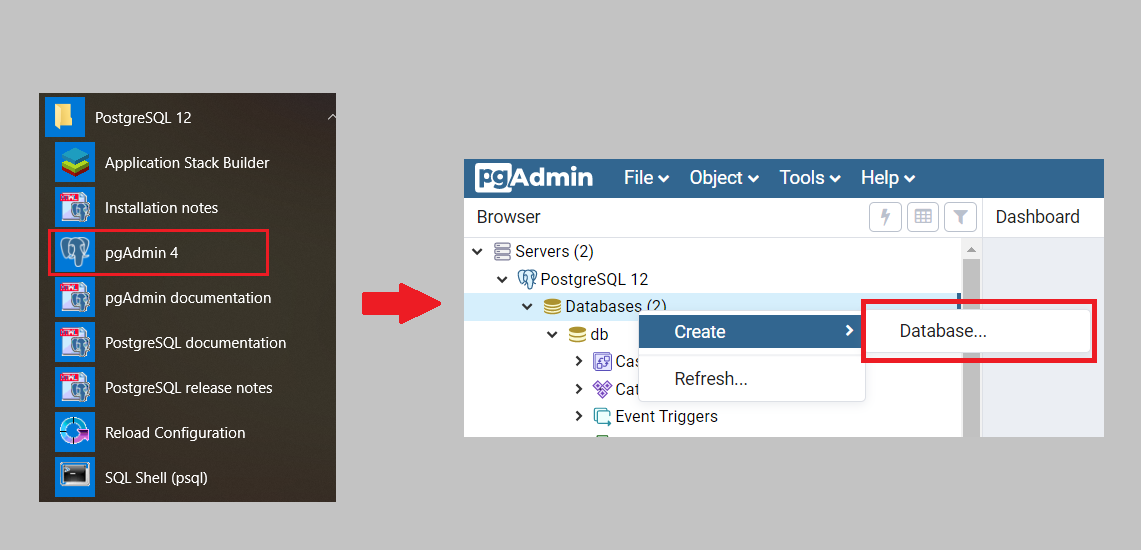
\includegraphics[scale=0.7]{slike/pustanjeupogon/a.png}
				\caption{Stvaranje baze podataka}
			\end{figure}
			
			Backend aplikacije pisan je u programskom jeziku Java, stoga računalo mora na sebi imati instaliran Java Development Kit(JDK) verzija 13. Preuzeti ga je moguće sa službene web stranice:
			\\
			\texttt{\small https://www.oracle.com/technetwork/java/javase/downloads/index.html}
			\\
			Provesti standardnu instalaciju i provjeriti je li sve ispravno instalirano tako da se otvori Command Prompt i upiše \textbf{\texttt{'java --version'}}, ako je sve uredu ispisati će se verzija instalirane jave.
			
			\begin{figure}[h]
				\centering
				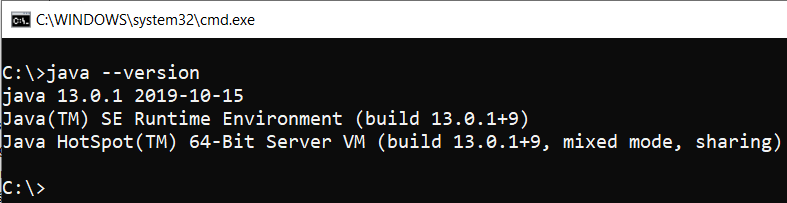
\includegraphics[scale=0.6]{slike/pustanjeupogon/javaversion.png}
				\caption{Provjera je li JDK ispravno instaliran}
			\end{figure}

			U pisanju backenda korišten je Spring framework te zato računalo mora imati instaliran Maven koji vodi računa o svim zavisnostima (dependencies) koje projekt ima. Potrebno je preuzeti zip arhivu s web stranice:
			\\
			\texttt{\small https://maven.apache.org/download.cgi}
			\\
			te ju raspakirati u željeni direktorij. Potom, podesiti environment varijable operacijskog sustava tako da otvorite \texttt{\textit{'System Properties'}} (to je moguće na par načina, ali najlakše je tako da se u polje za pretraživanje upiše: \texttt{\textit{'edit the system en...'}}) i odaberete \texttt{\textit{'Edit the system environment variables'}}.
			
			\begin{figure}[h]
				\centering
				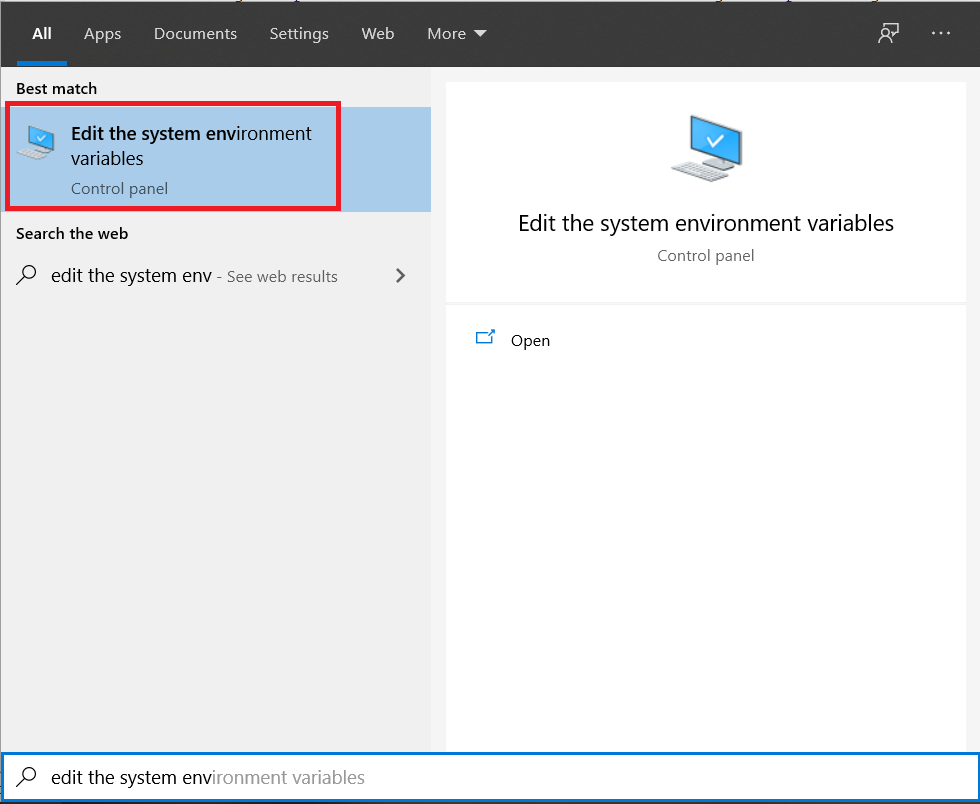
\includegraphics[scale=0.45]{slike/pustanjeupogon/search.png}
				\caption{Otvaranje System Properties}
			\end{figure}
			
			U prozoru koji se otvorio odaberite \texttt{\textit{'Environment Variables'}}, nakon toga odabrati opciju \texttt{\textit{'New'}} u dijelu sučelja \texttt{\textit{'System Variables'}}, u polje \texttt{\textit{'Variable name'}} upisati \texttt{\textit{'MAVEN\_HOME'}}, a u polje \texttt{\textit{'Variable value'}} upisati putanju direktorija koji je nastao raspakiravanjem zip arhive. Potom je potrebno odabrati opciju \texttt{\textit{'Edit'}} za varijablu \texttt{\textit{'Path'}} u polju \texttt{\textit{'System Variables'}} i kada se otvori novi prozor odabrati opciju \texttt{\textit{'New'}} te upisati \texttt{\small '\%MAVEN\_HOME\%\textbackslash bin'}. Maven bi sada trebao biti uspješno instaliran, provjeriti tako da se u Command Prompt upiše naredba \texttt{\textbf{'mvn --version'}}.
			
			\begin{figure}[h]
				\centering
				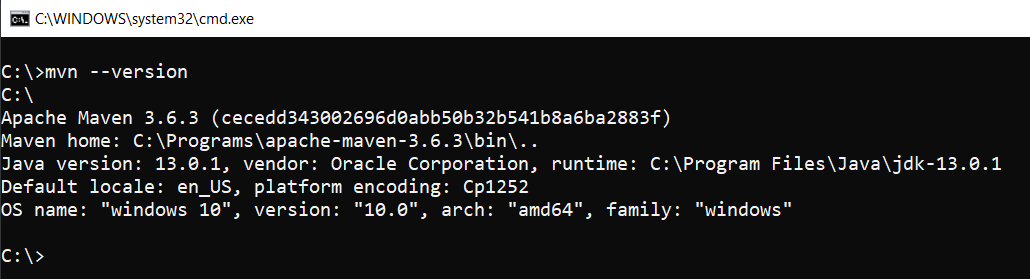
\includegraphics[scale=0.5]{slike/pustanjeupogon/mavenversion.png}
				\caption{Provjera je li Maven ispravno instaliran}
			\end{figure}
		
			Frontend aplikacije napisan je koristeći React Javascript library, stoga računalo mora imati instaliran Node.js kako bi ga mogli pokrenuti. S web stranice: 
			\\
			\texttt{\small https://nodejs.org/en/}
			\\
			preuzeti i pokrenuti installer datoteku. Provesti standardnu instalaciju. Provjeriti je li instalacija uspješna tako da se u Command Prompt upiše naredba \texttt{\textbf{'node --version'}}.
			
			\begin{figure}[h]
				\centering
				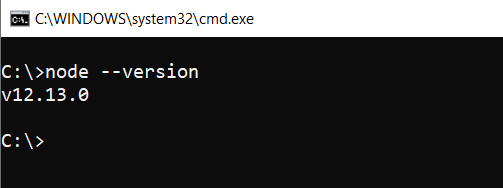
\includegraphics[scale=0.7]{slike/pustanjeupogon/nodeversion.png}
				\caption{Provjera je li Node.js ispravno instaliran}
			\end{figure}
		
			Sada kada su svi potrebni programi instalirani možemo početi s puštanjem aplikacije u pogon. Preuzeti direktorij s GitLab stranice:
			\\
			\texttt{\small https://gitlab.com/fermark/flow}
			\\
			tako da se odabere opcija \texttt{Download->zip}. Raspakirati zip arhivu te navigirati u direktorij \texttt{\small flow\textbackslash src\textbackslash main\textbackslash resources} te otvoriti datoteku \texttt{\textit{ application.properties}}. Potrebno je podesiti nekoliko parametara kako bi se moglo ispravno spojiti na bazu podataka. Za vrijednost parametra \texttt{\small <ime baze podataka>} u polju \texttt{\small spring.datasource.url} potrebno je upisati ime vaše baze podataka. U polja \texttt{\small username} i \texttt{\small password} upisati korisničko ime i lozinku koju ste odabrali kada ste instalirali PostgreSQL bazu podataka. Spremiti izmijene u datoteci.
			
			\begin{figure}[h]
				\centering
				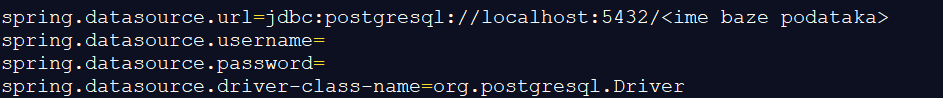
\includegraphics[scale=0.8]{slike/pustanjeupogon/app.png}
				\caption{Izmjena datoteke 'application.properties'}
			\end{figure}
			
			Otvoriti Command Prompt i navigirati u direktorij \texttt{\small \textbackslash flow} te tamo izvršiti naredbu \texttt{\textbf{'mvn install'}}. Time se stvorila izvršna datoteka tipa \texttt{'jar'} u poddirektoriju \texttt{\small target}. Sada je potrebno postaviti i frontend dio aplikacije. U Command Promptu navigirati u direktorij \texttt{\small \textbackslash flow\_front} te tamo izvršiti naredbu \texttt{\textbf{'npm install'}} koja će preuzeti biblioteku React. Potom u istome direktoriju je potrebno izvršiti naredbe \texttt{\textbf{'npm install react-router-dom --save'}} i \texttt{\textbf{'npm install axios --save'}}, a te dvije naredbe će preuzeti potrebne zavisnosti (dependecies) projekta.
			\\
			Sada još jedino preostaje pokrenuti aplikaciju. U direktoriju \texttt{\small \textbackslash flow\_front} izvršiti naredbu \texttt{\textbf{'npm start'}}, frontend dio aplikacije će se pokrenuti. Zatim je potrebno otvoriti novu instancu Command Prompta i u direktoriju \texttt{\small \textbackslash flow\textbackslash target} izvršiti naredbu \texttt{\textbf{'java -jar flow-0.0.1-SNAPSHOT.jar'}}. Ta će naredba pokrenuti backend dio aplikacije koji automatski stvara sve potrebne tablice u bazi podataka, jedino što je još potrebno napraviti je ubaciti u bazu podataka podatke za prijavu administratora. Ponovo pokrenuti sučelje za upravljanje bazom podataka \texttt{\textit{pgAdmin}} i pritisnuti desni klik na vašoj bazi podataka te odabrati opciju \texttt{\textit{Query Tool...}}.
			
			\begin{figure}[h]
				\centering
				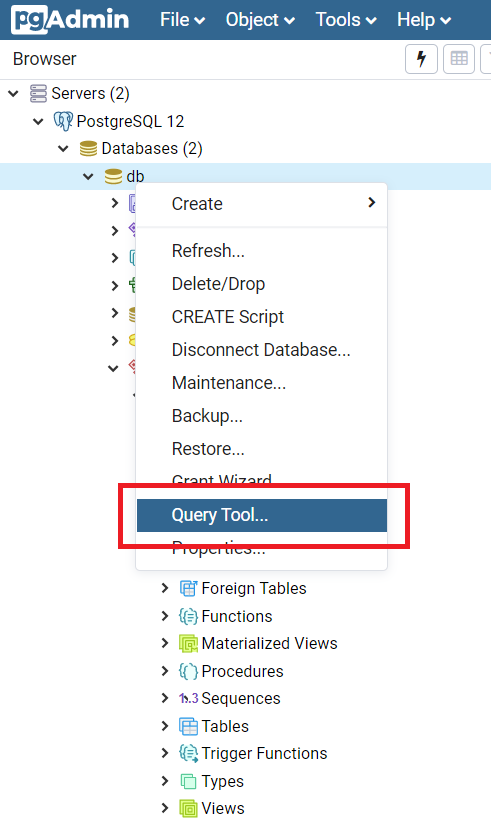
\includegraphics[scale=0.5]{slike/pustanjeupogon/query.png}
				\caption{Otvaranje Query Toola u pgAdmin sučelju}
				
			\end{figure}
			\newpage
			 U polje \texttt{\small Query Editor} upisati naredbu \texttt{\textbf{'INSERT INTO client VALUES ('1', 'ADMIN', 'ADMIN, 'ADMIN, 'ADMIN');'}} i izvršiti ju pritiskom na gumb s ikonom munje.
			
			\begin{figure}[h]
				\centering
				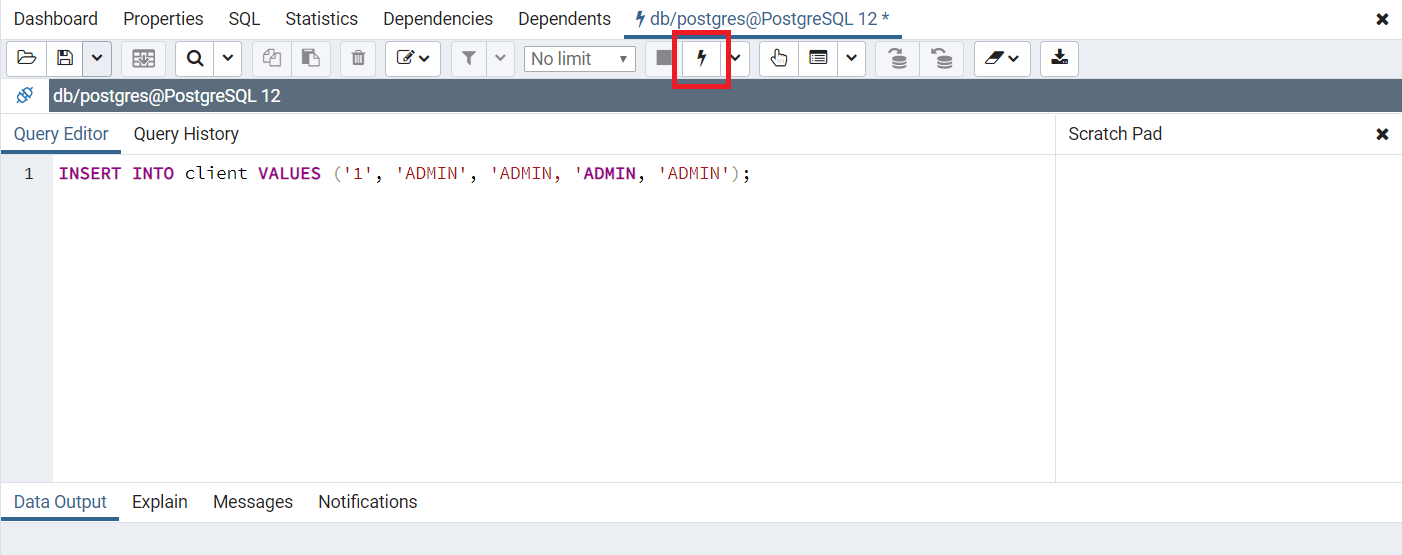
\includegraphics[scale=0.5]{slike/pustanjeupogon/insert.png}
				\caption{Izvršavanje naredbe u sučelju pgAdmin}
			\end{figure}
			
			Aplikacija je pokrenuta i moguće joj je pristupiti na URL
			\\
			\texttt{ \small http://localhost:3000/}
			
			
			\eject 